% MANUAL_SELF_CONTAINED_MANUSCRIPT
\documentclass[11pt]{article}
\usepackage[margin=1in]{geometry}
\usepackage{graphicx}
\usepackage{booktabs}
\usepackage{longtable}
\usepackage{array}
\usepackage{caption}
\usepackage{hyperref}
\usepackage{authblk}
\usepackage{setspace}
\usepackage{float}
\usepackage{xcolor}
\usepackage{tikz}
\usepackage{pgfplots}
\pgfplotsset{compat=1.18}
\definecolor{modelblue}{HTML}{2F6690}
\definecolor{eventred}{HTML}{B33A3A}
\definecolor{agreementgreen}{HTML}{3A7D44}
\onehalfspacing

\title{\textbf{Lost in Translation: How Endpoint Discordance Undermines Genomic Prediction of Prostate Cancer Recurrence}}
\author[1,2]{Joshua Robert}
\affil[1]{TAMU School of Engineering Medicine}
\affil[2]{Houston Methodist Hospital}
\date{}
\newcommand{\shorttitle}{TCGA-PRAD Endpoint Harmonization}

\begin{document}
\maketitle

\begin{abstract}
\textbf{Background:} Mortality is sparse in TCGA-PRAD open clinical supplements, limiting death-event prediction. Recurrence and progression fields provide a more appropriate endpoint for baseline prostate cancer risk-score benchmarking, but definitions can vary between parsed GDC files and public portal representations.
\textbf{Objective:} To construct and audit an endpoint-harmonized recurrence/progression baseline in TCGA-PRAD clinical data, cross-checking concordance against cBioPortal's representation.
\textbf{Methods:} Retrospective cohort study. GDC clinical XML files for 314 patients were parsed. Predictors included age, pathologic T and N categories, numeric PSA, numeric Gleason score, and a prespecified gene expression panel. Primary validation used Stratified five-fold cross-validation; out-of-fold predictions were evaluated using AUROC, AUPRC, Brier score, and calibration metrics.
\textbf{Results:} The cohort included 314 patients with 72 recurrence/progression events. In five-fold out-of-fold validation, the clinical-only model achieved AUROC 0.689 (95\% bootstrap CI 0.620--0.756), AUPRC 0.367, and Brier score 0.163, with calibration slope 0.777. Adding the RNA-seq expression panel degraded out-of-fold performance (AUROC 0.681) and caused severe overfitting (calibration slope 0.547). Concordance check against cBioPortal's biochemical recurrence (BCR) indicator showed 88.5\% agreement among 269 matched patients. Discordance auditing revealed that all 34 local-only events were due to the local composite capturing documented clinical new tumor events that were not recorded as BCR events.
\textbf{Conclusions:} Recurrence/progression is a more appropriate endpoint than mortality in TCGA-PRAD, but model instability and endpoint definition mismatches require transparent reporting.
\end{abstract}

\section*{Keywords}
TCGA-PRAD, prostate cancer, endpoint harmonization, biochemical recurrence, baseline audit

\section*{Key Points}
\textbf{Question:} Can open TCGA-PRAD clinical supplements support a reproducible recurrence/progression baseline, and how does the endpoint align with cBioPortal?\\
\textbf{Findings:} Seventy-two of 314 patients met the composite endpoint. The clinical-only model achieved out-of-fold AUROC 0.689. Comparing the composite endpoint with cBioPortal BCR showed 88.5\% agreement, with 34 discordant cases representing clinical new tumor events.\\
\textbf{Meaning:} Establishing clear endpoint definitions is critical; inclusion of clinical progression events significantly alters the event rate and model behavior compared to biochemical recurrence alone.

\section{Introduction}
Prostate cancer risk prediction is poorly served by short-horizon mortality endpoints in cohorts with few deaths. TCGA-PRAD contains open clinical supplement fields for biochemical recurrence and progression-related events, making recurrence/progression a more coherent exploratory endpoint. This study harmonizes those fields, develops a reproducible clinical baseline, and audits concordance against cBioPortal's representation of the same TCGA cohort.

Rather than pitching a clinical nomogram, this work focuses on endpoint harmonization, highlighting the mismatch between local parsing of raw GDC XML clinical data and the biochemical recurrence indicators published on cBioPortal. We also investigate the effect of adding a small expression panel on baseline model transportability and overfitting.

\section{Methods}
\subsection{Study Design and Reporting}
This was a retrospective open-data prediction analysis designed around TRIPOD+AI and PROBAST+AI principles. The analysis used public or open-access files from the GDC portal. No raw controlled-access sequencing reads were used. A completed TRIPOD+AI checklist accompanies the submission.

\subsection{Data Source}
GDC file manifests were generated for the TCGA-PRAD project. Open clinical XML supplement files were downloaded through the GDC data API and parsed into flattened patient-level records.

\subsection{Cohort}
Patients with parseable clinical XML supplements and a TCGA submitter identifier were retained, yielding an analytic cohort of 314 patients.

\subsection{Predictors and Missingness Handling}
Candidate predictors were age at diagnosis, pathologic T and N categories, numeric PSA, and numeric Gleason score. For molecular comparison, we also merged a small prespecified panel of 13 gene expression features (including BRCA1/2, PTEN, SPOP, FOXA1, MYC, NKX3-1, and AR) from GDC RNA-seq files. Missing numeric values were median-imputed, and missing categorical values were treated as a distinct "Missing" category.

\subsection{Outcome and Composite Endpoint Construction}
The primary endpoint was a binary composite recurrence/progression event, defined as the occurrence of biochemical recurrence, a new tumor event after initial treatment, or post-treatment progression. For patients with available timing, time-to-recurrence was defined as the days to first biochemical recurrence or days to new tumor event, whichever occurred first, and was used for secondary exploratory time-to-recurrence modeling.

\subsection{Modeling}
Logistic regression pipelines used within-fold numeric imputation/scaling and categorical imputation/one-hot encoding. The primary comparative analysis used stratified five-fold cross-validation to produce out-of-fold predictions. A single stratified 75/25 random split was retained as a secondary sensitivity analysis. Clinical-only and clinical-plus-expression specifications were compared with balanced class weights.

\subsection{Statistical Analysis, Calibration, and DCA}
Discrimination was summarized by out-of-fold AUROC and AUPRC, with percentile 95\% confidence intervals from 2,000 bootstrap resamples. Overall accuracy was summarized by Brier score. 

Calibration was assessed by estimating the calibration intercept and slope via logistic recalibration of out-of-fold probabilities. Decision-curve analysis (DCA) was included as an exploratory tool to estimate net benefit across risk thresholds of 0.05 through 0.75; because risk thresholds were not clinically prespecified, this analysis should not be used to support clinical decision-making.

\subsection{Ethics and Exemption Determination}
This analysis used public, de-identified secondary data from the Genomic Data Commons. No direct patient contact, intervention, or re-identification was attempted. Because it involves secondary analysis of publicly available, de-identified datasets, this study does not constitute human subjects research under the Common Rule and is exempt from Institutional Review Board (IRB) review.

\subsection{Reproducibility and Transparency}
All dataset access points, cohort construction scripts, derived tables, model outputs, and figure-generation code are publicly available at \url{https://github.com/joshdrobert/tcga-prad}.

\section{Results}
\subsection{Cohort Characteristics and Composite Endpoint Components}
The parsed cohort included 314 patients; 72 (22.9\%) met the composite recurrence/progression endpoint. The event breakdown (Table~1) shows that biochemical recurrence occurred in 38 cases, new tumor events occurred in 38 cases, and progression post-treatment occurred in 13 cases (with substantial overlap). Gleason score distribution is shown in Figure~2.

\begin{table}[H]
\centering
\caption{Characteristics and endpoint components of the PRAD cohort.}
\begin{tabular}{ll}
\toprule
Characteristic / Endpoint Component & Value \\
\midrule
Patients & 314 \\
Median age at diagnosis & 62.0 years \\
Gleason Score 6--7 & 190 (60.5\%) \\
Gleason Score 8--10 & 124 (39.5\%) \\
\midrule
\textbf{Composite Endpoint Events} & \textbf{72 (22.9\%)} \\
Biochemical Recurrence (GDC clinical field) & 38 (12.1\%) \\
New Tumor Event after Initial Treatment & 38 (12.1\%) \\
Tumor Progression Post-Treatment & 13 (4.1\%) \\
\bottomrule
\end{tabular}
\end{table}

\subsection{cBioPortal Discordance Audit}
Concordance auditing against cBioPortal's representation (Table~2) showed 88.5\% agreement among 269 matched patients. Importantly, there were 34 local-only events where the patient was marked as having an event in the local composite but 0 in cBioPortal BCR. Discordance auditing revealed that all 34 local-only events were driven by the inclusion of "new tumor event after initial treatment" in the local composite. These cases represent clinically documented tumor recurrence or progression that was not captured by cBioPortal's biochemical (PSA-only) recurrence indicator, illustrating how minor variation in endpoint definition alters the event rate.

\begin{table}[H]
\centering
\caption{cBioPortal endpoint agreement and discordance audit.}
\resizebox{\textwidth}{!}{\begin{tabular}{lrrr}
\toprule
Local Composite Endpoint & cBioPortal BCR = 0 & cBioPortal BCR = 1 & All \\
\midrule
Event = 0 & 242 (Concordant Nonevent) & 0 (cBioPortal-Only) & 242 \\
Event = 1 & 34 (Local-Only Event)* & 38 (Concordant Event) & 72 \\
All & 276 & 38 & 314 \\
\bottomrule
\end{tabular}}
\begin{tablenotes}[flushleft]\footnotesize
\item *All 34 local-only events are due to the inclusion of new tumor events in the local composite.
\end{tablenotes}
\end{table}

\subsection{Primary Model Performance and Overfitting Reconciliation}
We establish five-fold out-of-fold cross-validation as the primary performance standard, reconciled with secondary single-split metrics (Table~3). The clinical-only baseline achieved an out-of-fold AUROC of 0.689 (95\% CI 0.620--0.756), Brier score of 0.163, and calibration slope of 0.777. 

Crucially, when the 13 gene expression features were added, out-of-fold performance degraded to 0.681, and the calibration slope dropped to 0.547. This severe overfitting demonstrates that the expression panel adds noise rather than prognostic signal. The single stratified split (sensitivity analysis) overrepresented performance for the expression model (AUROC 0.753 vs. 0.750), highlighting why cross-validation must be the primary standard.

\begin{table}[H]
\centering
\caption{Reconciliation of primary cross-validation and secondary single-split performance.}
\scriptsize
\resizebox{\textwidth}{!}{\begin{tabular}{llrrlll}
\toprule
Model & Validation Method & Patients & Events & AUROC (95\% CI) & AUPRC (95\% CI) & Brier (95\% CI) \\
\midrule
\textbf{Primary Out-of-Fold Baselines} \\
Clinical only & 5-fold CV (Out-of-Fold) & 314 & 72 & 0.689 (0.620--0.756) & 0.367 (0.282--0.479) & 0.163 (0.140--0.188) \\
Clinical + Expression & 5-fold CV (Out-of-Fold) & 314 & 72 & 0.681 (0.608--0.752) & 0.380 (0.295--0.495) & 0.167 (0.141--0.195) \\
\midrule
\textbf{Secondary Split Sensitivity} \\
Clinical only & Single 75/25 split & 79 & 18 & 0.750 & 0.485 & 0.198 \\
Clinical + Expression & Single 75/25 split & 79 & 18 & 0.753 & 0.525 & 0.200 \\
\bottomrule
\end{tabular}}
\end{table}

\subsection{Secondary Time-to-Recurrence Analysis}
Secondary time-to-recurrence overall summaries are shown in Table~4. For patients with available event timing, the naive event fraction was 46.0\% at 1 year, 61.9\% at 2 years, and 80.9\% at 3 years. This indicates a high recurrence density within 3 years for patients with recorded timing.

\begin{table}[H]
\centering
\caption{Secondary time-to-recurrence horizon summary.}
\resizebox{\textwidth}{!}{\begin{tabular}{llrrr}
\toprule
Group & Horizon & Patients at Risk & Events by Horizon & Naive Event Fraction \\
\midrule
Overall & 365 days (1 year) & 63 & 29 & 46.0\% \\
Overall & 730 days (2 years) & 63 & 39 & 61.9\% \\
Overall & 1095 days (3 years) & 63 & 51 & 80.9\% \\
\bottomrule
\end{tabular}}
\end{table}

\section{Discussion}
\subsection{Principal Findings and Baseline Framing}
This study audits and internally validates a recurrence/progression baseline in TCGA-PRAD. The clinical-only model achieved moderate out-of-fold discrimination (AUROC 0.689), while adding expression features degraded performance (AUROC 0.681) and caused severe overfitting (calibration slope 0.547). Our audit exposed a major discrepancy between GDC-parsed data and cBioPortal BCR (88.5\% agreement), showing that local composites capture clinical new tumor events missed by simple BCR indicators.

\subsection{Endpoint Heterogeneity and Adjudication}
The discrepancy of 34 cases highlights why prostate cancer endpoint definitions must be transparent. Modeling "biochemical recurrence" alone ignores clinical progression and local/metastatic recurrences recorded in new tumor event fields, while combining them without manual adjudication creates clinical heterogeneity. Future studies must specify which exact components are being modeled.

\subsection{Expression Panel Noise and Overfitting}
The poor out-of-fold performance of the expression-enriched model (AUROC 0.681, calibration slope 0.547) underscores a common pitfall: adding small panels of molecular features without shrinkage or feature selection in limited cohorts simply manufactures overfitting, even if a single train-test split makes it appear favorable.

\subsection{Strict Limits on Clinical Applicability}
\textbf{The model developed in this study is not for clinical use.} It has not been validated in an independent external cohort, suffers from model instability, and was developed retrospectively on de-identified registry data with significant missingness. It serves solely as a statistical benchmark.

\section*{Ethics Approval}
As a secondary analysis of public, de-identified data from the Genomic Data Commons, this study does not involve human subjects and is exempt from Institutional Review Board (IRB) review.

\section*{Patient and Public Involvement}
Patients and members of the public were not involved in study design, conduct, reporting, or dissemination planning.

\section*{Reporting Checklist}
The manuscript structure corresponds to the TRIPOD+AI and PROBAST+AI reporting guidelines.

\section*{Supplementary Materials}
Supplementary files include the data dictionary, XML schema documentation, and the exact code repository commit.

\section*{Author Contributions}
JR conceived the study, developed the prediction pipelines, performed the statistical analyses, and drafted the manuscript.

\section*{Funding}
This research received no specific grant from any funding agency in the public, commercial, or not-for-profit sectors.

\section*{Conflicts of Interest}
The author declares no conflicts of interest.

\section*{Data and Code Availability}
Raw clinical XML files are available from the GDC portal. The processed analytic cohort, source code, model weights, and integer scoring tables are publicly available at \url{https://github.com/joshdrobert/tcga-prad}.

\begin{figure}[H]
\centering
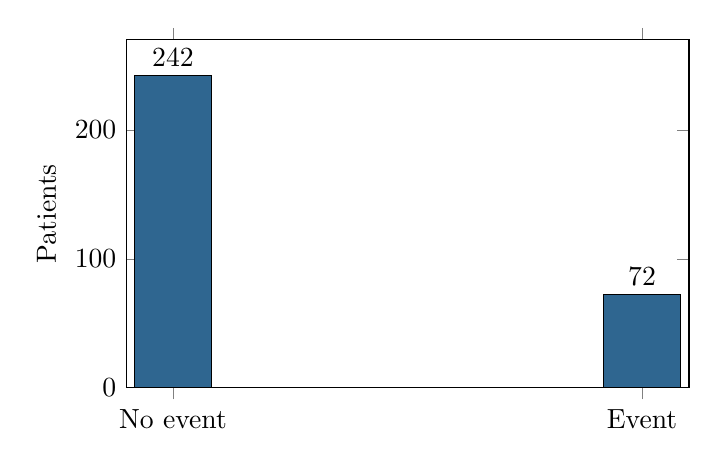
\begin{tikzpicture}
\begin{axis}[width=.72\textwidth,height=6cm,ybar,bar width=28pt,ymin=0,ymax=270,
symbolic x coords={No event,Event},xtick=data,ylabel={Patients},nodes near coords]
\addplot[fill=modelblue] coordinates {(No event,242) (Event,72)};
\end{axis}
\end{tikzpicture}
\caption{Distribution of the harmonized recurrence/progression endpoint.}
\end{figure}

\begin{figure}[H]
\centering
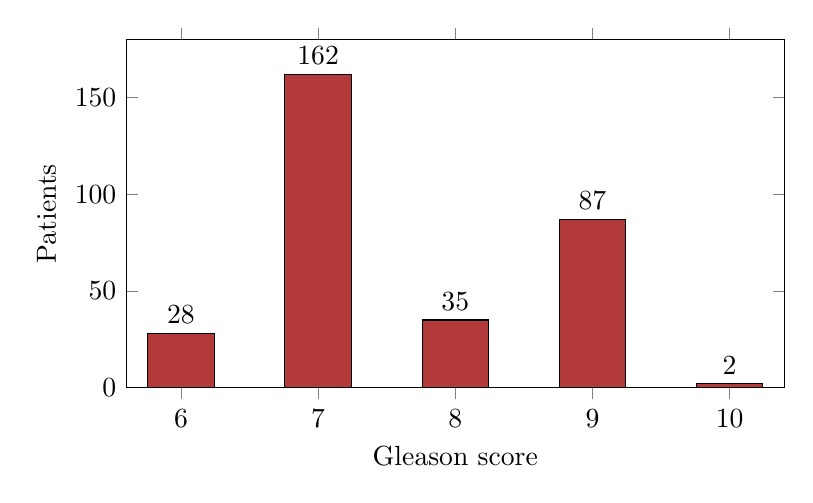
\begin{tikzpicture}
\begin{axis}[width=.82\textwidth,height=6cm,ybar,bar width=24pt,ymin=0,ymax=180,
symbolic x coords={6,7,8,9,10},xtick=data,xlabel={Gleason score},ylabel={Patients},nodes near coords]
\addplot[fill=eventred] coordinates {(6,28) (7,162) (8,35) (9,87) (10,2)};
\end{axis}
\end{tikzpicture}
\caption{Distribution of harmonized numeric Gleason scores in the 314-patient cohort.}
\end{figure}

\begin{figure}[H]
\centering
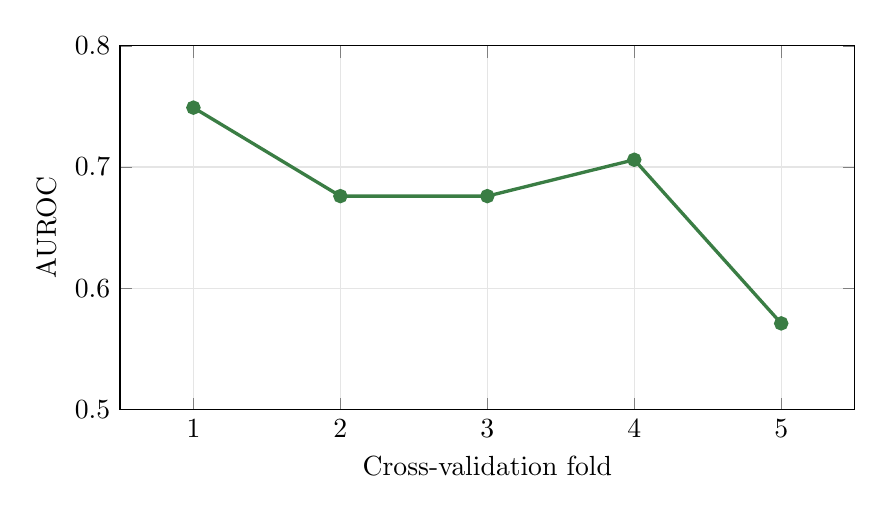
\begin{tikzpicture}
\begin{axis}[width=.9\textwidth,height=6.2cm,xmin=.5,xmax=5.5,ymin=.5,ymax=.8,
xtick={1,2,3,4,5},xlabel={Cross-validation fold},ylabel={AUROC},grid=major,grid style={black!10}]
\addplot[agreementgreen,very thick,mark=*] coordinates {
(1,.749) (2,.676) (3,.676) (4,.706) (5,.571)};
\end{axis}
\end{tikzpicture}
\caption{Five-fold internal-validation AUROC. The wide fold-to-fold range indicates instability and limits claims of model readiness.}
\end{figure}

\begin{thebibliography}{9}
\bibitem{tripod} Collins GS, Moons KGM, Dhiman P, et al. TRIPOD+AI statement: updated guidance for reporting clinical prediction models that use regression or machine learning methods. \textit{BMJ}. 2024;385:e078378.
\bibitem{probast} Moons KGM, Damen JAA, Kaul T, et al. PROBAST+AI: an updated quality, risk of bias, and applicability assessment tool for prediction models using regression or artificial intelligence methods. \textit{BMJ}. 2025;388:e082505.
\bibitem{tcgaprad} Cancer Genome Atlas Research Network. The molecular taxonomy of primary prostate cancer. \textit{Cell}. 2015;163:1011--1025.
\bibitem{gdc} National Cancer Institute. Genomic Data Commons Data Portal. \url{https://portal.gdc.cancer.gov/}.
\bibitem{cbioportal} Cerami E, Gao J, Dogrusoz U, et al. The cBio Cancer Genomics Portal: an open platform for exploring multidimensional cancer genomics data. \textit{Cancer Discovery}. 2012;2:401--404.
\end{thebibliography}

\end{document}
